\documentclass[../main.tex]{subfiles}

\begin{document}

\chapter[Resilient Primal Decomposition-based dMPC]{Resilient \\Primal Decomposition-based \\distributed \\Model Predictive Control}\label{sec:safe_pddmpc_ineq}
\epigraph{\centering Desperate times call for desperate measures}
{\textit{Title}\\\textsc{Author}}

In this chapter, we carry on the work from the last chapter relaxing some assumptions to make the problem to be solved more generic.
We apply the primal decomposition to the problem, and then, we compare the cases when the system presents nominal behavior and when the system is under the proposed attack model.

From the analysis, we notice how the relaxation of the assumption increases drastically the complexity of the problem.

Employing some assumptions, we take a powerful tool of our identification utility belt, and use it to create an approach to circumvent the complexity of the system, allowing us to adapt the detection and mitigation presented in the last chapter.

\minitoc

\section{Relaxing the problem}\label{sec:not-so-scarce}
We begin again with the monolithic \mpc{} equivalent problem~\eqref{eq:qp_standard_form}.
We reproduce yet another time the problem, but with a twist, now the problem also has a decomposable constraint set $\set{U}$:
\begin{equation}
  \label{eq:qp_standard_form_again_set_constraint}
  \begin{aligned}
    \begin{matrix}
      \minimize\limits_{\vec{U}[k]} &
                                      \frac{1}{2}\norm{\vec{U}[k]}^{2}_{H} + {\vec{f}[k]}^{T}\vec{U}[k] &\\
      \mathrm{subject~ to} & \bar{\Gamma}\vec{U}[k]\preceq {\vec{U}}_{\text{max}} \\
                                    & \vec{U}[k]\in \set{U}
    \end{matrix}
  \end{aligned}.
\end{equation}
We decompose the system using the primal decomposition, and the local problems also have constraint sets, denoted $\set{U}_{i}$:
\begin{equation}
  \label{eq:DOP_local_set_constraint}
  \eqoptobji(\thetaik)[k]=
  \begin{matrix}
    \minimize\limits_{\vec{U}_{i}[k]}&\frac{1}{2}\norm{\vec{U}_{i}[k]}^{2}_{H_{i}} + {\vec{f}_{i}[k]}^{T}\vec{U}_{i}[k]\\
    \mathrm{subject~ to} & \bar{\Gamma}_{i}\vec{U}_{i}[k] \preceq \thetaik:\lambdaik\\
                                     & \vec{U}_{i}[k]\in \set{U}_{i}
  \end{matrix},
\end{equation}
and we use the projected subgradient method~\eqref{eq:projectedSubgradient_lambda} (reproduced for convenience) to solve the main problem:
\begin{equation}
  \label{eq:projectedSubgradient_lambda_reprise}
  \tag{\ref*{eq:projectedSubgradient_lambda}}
  \vec{\theta}[k]\pplusone=\Proj^{\set{S}}(\vec{\theta}[k]\p+\rho\p\vec{\lambda}[k]\p),
\end{equation}
but with ${\set{S} = \setbuild{\vec{\theta}[k]}{I_{c}^{M}\vec{\theta}[k]\preceq \vec{U}_{\max}}}$.
\begin{remark}
  As seen in~\cite{BoydEtAl2015}, if we have separable constraints sets, such as the $\set{U}_{i}$ in our problem, we can modify the local objectives $\obji$ so \begin{equation*}
    J_{i}(\optthetai)=\infty\text{, if }\vec{U}_{i}^{\star}\notin\dom{\obji}.
  \end{equation*}
  Since this change modifies the objective functions, it also modifies the corresponding gradients, and $\lambdai$ as consequence.
  So, this change guides the coordinator to choose $\thetai$ which respect $\dom{\obji}$.
\end{remark}

In this chapter, we still assume the original constraint~\eqref{eq:linear_constraint} to have at most as many rows as columns, i.e., $\card{\vec{u}_{\max}}\leq n_{u}$.
However, we relax the assumption made in \S\ref{sec:scarce-systems}.
The systems are not necessarily scarce anymore, i.e., the unconstrained solutions
$\optuncU=-H^{-1}\vec{f}[k]$ and $\optuncUik=-H_{i}^{-1}\vec{f}_{i}[k]$ may or may not respect the constraints.

As we will see in next section, despite the relaxation of this assumption, making the problem more generic, it causes the solution of the local problems exponentially more complex.

\section{Impact on local problems' solution}\label{sec:impact-local-problem}
We can repeat the analysis made in the last chapter to see how the change on assumption influences the solutions of the problem.

Although now we have \qp{} problems with inequality constraints, we still can use the same method to find a analytical solution.

We similarly define a function $\inequalityfunctionname:\R^{\card\vec{U}_{i}[k]}\times \R^{\card\thetaik}$:
\begin{equation}
  \label{eq:lagrangian_inequality}
  \inequalityfunction=\bar{\Gamma}_{i}\vec{U}_i[k]-\thetaik,
\end{equation}
and use it to put the problem in standard form for inequality constraint \qp{} programs:
\begin{equation}
  \begin{matrix}
    \label{eq:local_problem_equality_standard_notation}
    \minimize\limits_{\vec{U}_{i}[k]}&\obji(\vec{U}_{i}[k],\thetaik)\\
    \mathrm{subject~ to} & \inequalityfunction\preceq 0:\lambdaik
  \end{matrix},
\end{equation}
with variables $\lambdaik$ associated to the constraints.
\begin{remark}
  Usually we make the distinction between the dual variables associated to the inequality and equality constraints by using different symbols.
  However, as in the problems we have only one kind, we use the same symbol and by context the reader can distinguish to which kind the symbol corresponds.
\end{remark}

We can again define the \emph{Lagrangian} function $\lagrangianname : \R^{\card\vec{U}_{i}[k]}\times \R^{\card\lambdaik} \times \R^{\card\thetaik} \to \R$ as
\begin{equation}
  \label{eq:lagrangian_equality}
  \lagrangian=\obji(\vec{U}_{i}[k],\thetaik)+\lambdaik^T\inequalityfunction,
\end{equation}
which embeds the inequality constraint into the objective function using $\lambdaik$, in this case the lagrangian multiplier for \emph{inequality}.
Again, since there is only one type of lagrangian multiplier, we will call it simply as the dual variable.

\begin{remark}
  The complementary slackness still holds, ${\lambdaikstar}^T\inequalityfunctionname(\vec{U}_{i}^{\star}[k],\thetaik)$ will always be zero.
  If any element of $\inequalityfunctionname(\vec{U}_{i}^{\star}[k],\thetaik)$ is smaller than zero, the corresponding element on the dual variable $\lambdaikstar$ will be zero, indicating the constraint is active.
\end{remark}

We can define the dual function $\dualfunctionname:\R^{\card\lambdaik} \times \R^{\card\thetaik} \to \R$ also calculated by solving
\begin{equation}
  \label{eq:dual_function_equality}
  \dualfunction=\inf_{\vec{U}_{i}[k]\in\set{F}} \lagrangian,
\end{equation}
but now where $\set{F}=\dom \inequalityfunctionname=\bigcap\limits_{i=1}^{\card\vec{U}_{\max}}\set{H}_{i}$, with $\set{H}_{i}$ being the halfspaces
${\set{H}_i=\setbuild{\vec{x}}{\elem[i,\star]{{\bar{\Gamma}}}\vec{x}\leq\elem[i,\star]{\vec{U}_{\max}}}}$.
Using the first order \KKT{} optimality condition we have
\begin{equation}
  \nabla_{\vec{U}_{i}[k]}\lagrangian=0
\end{equation}
yielding as well
\begin{equation}
  \vec{U}_{i}[k]=-H_{i}^{-1}\vec{f}_{i}[k]+H_{i}^{-1}\bar{\Gamma}_{i}^{T}\lambdaik,
\end{equation}
which we know is
\begin{equation}
  \vec{U}_{i}[k]=\optuncUik-H_{i}^{-1}\bar{\Gamma}_{i}^{T}\lambdaik.
\end{equation}

Substituting it in $\lagrangian$ results
\begin{equation}
  \label{eq:dual_function_solution_lambda_theta_ineq}
  \dualfunction=-\frac{1}{2}\lambdaik^{T}\linearcoefi\lambdaik-\lambdaik^{T}\bar{\Gamma}_{i}H_{i}^{-1}\vec{f}[k]-\lambdaik^{T}\thetaik,
\end{equation}
which is also concave.

Then, similarly we can find $\lambdaikstar$ by solving an optimization problem.
However, since we are using inequalities, we can only have $\lambdaik$ positive~\cite{BoydVandenberghe2004}:
\begin{equation}
  \label{eq:ineq_lambda_equation}
  \begin{matrix}
    \lambdaikstar=\argmax\limits_{\lambdaik}\left\{
    \begin{matrix}
      \maximize\limits_{\lambdaik}&\dualfunction\\
      \mathrm{subject~ to}& \lambdaik\preceq\0
    \end{matrix}\right\}.
  \end{matrix}
\end{equation}

As we know, by complementary slackness, the value of the elements of $\lambdaik$ being $0$ (or different of $0$) will depend on the status of the corresponding constraint for the unconstrained solution $\optuncUik$.
So the complete value of $\lambdaik$ will depend of the permutation of the status of the inequality constraint.
Depending on the form of the constraints, if we have $\nineq$ constraints, we may have potentially $2^{\nineq}$ permutations.
\begin{remark}
  Here we say potentially because not necessarily all combinations are possible.
  In \S\ref{sec:cons-about-stat} we discuss briefly about the number of permutations and show some cases where the number of permutations is not equal to $2^{\nineq}$.
\end{remark}

To solve~\eqref{eq:ineq_lambda_equation}, we can use the fact that the status of the constraints depends on the value of $\thetaik$.
This way, we can notice that the set of constraints divides the space of $\thetaik$ into multiple regions denoted $\set{R}_{\lambdai}^{n}$, depending if the constraints are active or not for $\optuncUik$.

The regions $\set{R}_{\lambdai}^{n}$ are polytopes defined as ${\set{R}_{\lambdai}^{n}=\setbuild{\vec{x}}{G^{n}[k]\vec{x} \preceq b^{n}[k]}}$ where the hyperplanes may vary with time $k$.
As remarked in~\cite{BemporadEtAl2002}, the polytopes are non-overlapping, i.e., ${\set{R}_{\lambdai}^{i}\cap\set{R}_{\lambdai}^{j}=\emptyset, \forall i\neq j}$.
This way, the regions form a partition of the $\thetai$ space, i.e., given $\thetaik\in\set{Y}\subseteq\R^{\card{\thetaik}}$, ${\bigcup_{i\in\{0:\nineq-1\}}\set{R}^{i}=\set{Y}}$.
\begin{remark}
  Determining the exact polytopes/halfspaces is not in the scope of this work.
  But can be carried out by the methods in~\cite[\S4.1.3.2]{LauerBloch2019}.
\end{remark}

Imagine an example where we have $2$ constraints with associated $\elem[1]{\lambdai}$ and $\elem[2]{\lambdai}$, the $\thetai$ solution space is partitioned like in Fig.~\ref{fig:constraints_partition_theta} (indices $[k]$ suppressed for brevity).
\begin{figure}[h]
  \centering
  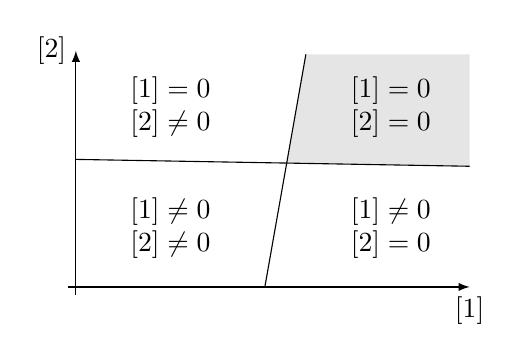
\begin{tikzpicture}[every node/.style={align=center}]
    \def\height{3}
    \def\length{5}
    \node at (0,0) {} coordinate (p0)  ++(0:\length*2.4/5) coordinate (p1) ;
    \node at (0,0) {} ++(90:\height*2.7/5) coordinate (p2) ;

    \draw[black] (p2) ++(-1:5) coordinate (p3);
    \draw[black] (p1) ++(80:3) coordinate (p4);
    \coordinate (p6) at (p3|-p4);

    \coordinate (p5) at (intersection cs:first line={(p2)--(p3)}, second line={(p1)--(p4)});
    \path[fill=gray!20] (p6) -- (p4) -- (p5) -- (p3);
    \draw[black] (p2) -- (p3);
    \draw[black] (p1) -- (p4);

    \draw[-latex] (0,-.1) - - (0,\height) node[left]{$\elem[2]{\thetai}$};
    \draw[-latex] (-.1,0) - - (\length,0) node[below]{$\elem[1]{\thetai}$};

    \node at (\length*1.2/5,\height*1.25/5) {$\elem[1]{\lambdai}\neq0$\\$\elem[2]{\lambdai}\neq0$};
    \node at (\length*1.2/5,\height*3.8/5) {$\elem[1]{\lambdai}=0$\\$\elem[2]{\lambdai}\neq0$};
    \node at (\length*4/5,\height*1.25/5) {$\elem[1]{\lambdai}\neq0$\\$\elem[2]{\lambdai}=0$};
    \node at (\length*4/5,\height*3.8/5) {$\elem[1]{\lambdai}=0$\\$\elem[2]{\lambdai}=0$};
  \end{tikzpicture}
  \caption{Two constraints partitioning $\thetai$ solution space.}\label{fig:constraints_partition_theta}
\end{figure}
For any $\thetai$ inside the grey area, the solution to~\eqref{eq:local_problem_equality_standard_notation} will be unconstrained, i.e., the constraint will be active.
Thus, for this case, by definition the value of $\lambdai=\0$.
For all other cases, where we know at least one constraint in~\eqref{eq:local_problem_equality_standard_notation} is inactive, we can remove the constraint in~\eqref{eq:ineq_lambda_equation} for the element of $\lambdai$ corresponding to the inactive constraint.
For instance, if all constraints in~\eqref{eq:local_problem_equality_standard_notation} are inactive, we can remove all constraints of~\eqref{eq:ineq_lambda_equation}, which will result in problem~\eqref{eq:eq_lambda_equation}, whose solution we known already:
\begin{equation}
  \label{eq:lambda_function_theta_reprise}
  \tag{\ref*{eq:lambda_function_theta}}
  \lambdaik=-\Plin\thetaik-\sik,
\end{equation}
\newcommand{\Plinineqnonzero}[1][\star]{\overset{#1}{\Plin}}
\newcommand{\sikineqnonzero}[1][\star]{\overset{#1}{\vec{s}_{i}}[k]}

By removing a set of constraints, we can solve a similar problem, but with reduced number of elements in $\thetai$ and $\lambdai$.
For example, let us suppose the first constraint in~\eqref{eq:local_problem_equality_standard_notation} is active.
We make $\elem[1]{\lambdai}=0$ and set it aside, we remove the corresponding lines of $\bar{\Gamma}_{i}$ and $\thetai$, and then we solve for all other elements of $\lambdai$, removing the remaining constraints in~\eqref{eq:ineq_lambda_equation}. This results in
\begin{equation}
  \label{eq:lambda_function_theta_some_active}
  \elem[2:\elemend]{\lambdai}[k]=-\Plinineqnonzero[2:\card{\lambdai}] \elem[2:\elemend]{\thetai}[k]-\sikineqnonzero[2:\card{\lambdai}],
\end{equation}
where $\Plinineqnonzero[2:\card{\lambdai}]={(\linearcoefiineqnonzero[2:\elemend,\star])}^{-1}$ and $\sikineqnonzero[2:\card{\lambdai}]=\Plinineqnonzero[2:\card{\lambdai}]\elem[2:\elemend,\star]{\bar{\Gamma}_{i}}H_{i}^{-1}\vec{f}_{i}[k]$.

If we do this for all partitions, i.e., all possible permutations of active and inactive constraints, we will have as many equations similar to~\eqref{eq:lambda_function_theta_some_active} as permutations.
This result is the base for calculating the solution of the original problem~\eqref{eq:local_problem_equality_standard_notation} as shown in~\cite{BemporadEtAl2002,AlessioBemporad2009}, which is the base for explicit \mpc{}.

However, the equations have different sizes of elements (as many elements as inactive constraints).
To make all equations same-sized, we recover the elements of $\lambdai$ set to zero and set aside.
If we take the same example, Eq.~\eqref{eq:lambda_function_theta_some_active} would become
\begin{equation}
  \label{eq:lambda_function_theta_some_active_same_size}
  \lambdaik=
  \left[
    \begin{matrix}
      0\\
      \elem[2:\elemend]{\lambdai}[k]
    \end{matrix}
  \right]
  =
  -
  \left[
    \begin{matrix}
      0&0\\
      0&\Plinineqnonzero[2:\card{\lambdai}]
    \end{matrix}
  \right]
  \thetaik
  -
  \left[
    \begin{matrix}
      0\\
      \sikineqnonzero[2:\card{\lambdai}]
    \end{matrix}
  \right]
\end{equation}


To facilitate the notation, let us use a binary representation such if we have $\nineq$, we use $\nineq$ binary digits to represent the active constraints.
And we will mark the digtis $1$ if the constraint is active and $0$ if inactive, indicating which constraints were removed or kept.

If we retake the $2$-constraints example in Fig.~\ref{fig:constraints_partition_theta}, ${00}_{(2)}$ would represent both constraints inactive (bottom left quadrant), ${01}_{(2)}$ and ${10}_{(2)}$ represents one of the constraints are active (bottom right and top left quadrants, respectively) and ${11}_{(2)}$ where both constraints are active (grey area in top right quadrant).
We can then use the base 10 to represent such partitions.
This way~\eqref{eq:lambda_function_theta_some_active_same_size} can be written as
\begin{equation}
  \label{eq:lambda_function_theta_same_size_coded}
  \lambdaik=-\Plin^{(2^{n_{\text{ineq}-1}})}\thetaik-\sik^{(2^{n_{\text{ineq}-1}})},
\end{equation}
with index $(2^{n_{\text{ineq}-1}})$ indicating that only the first constraint is active.

Then, we can write the complete solution of~\eqref{eq:ineq_lambda_equation} as
a \pwa{} function
\begin{equation}
  \label{eq:lambdafuntheta}
  \begin{aligned}
    \lambdaik=
    \begin{cases}
      -\Plinineq\thetaik-\sikineq,&\text{if}\ \thetaik \in\set{R}_{\lambdai}^{n}\\
      \qquad\quad \vdots&\qquad\quad \vdots\\
      -\Plinineq[i][2^{\nineq}-1]\thetaik-\sikineq[i][2^{\nineq}-1],&\text{if}\ \thetaik \in\set{R}_{\lambdai}^{2^{\nineq}-1}\\
    \end{cases}
  \end{aligned}.
\end{equation}

Here we can begin to regard the change caused by the relaxation, whereas we had only one equation relating $\lambdai$ to $\thetai$, when the system was scarce, now we have potentially $2^{\nineq}$ different equations.

\begin{remark}\label{rem:sparse_solutions}
  As one may expect, by definition, the $\Plinineq[i][n]$ and $\sikineq[i][n]$ are increasingly sparse, that means, as $n$ increases more constraints are active and more blocks are equal to zero, culminating in $\Plinineq[i][2^{\nineq}-1]=0_{\card{\lambdai}}$ and $\sikineq[i][2^{\nineq}-1]=\0_{\card{\lambdai}}$.
\end{remark}
\subsection{Considerations about status of constraints}\label{sec:cons-about-stat}
It is important to observe that some there are some sets of constraints in which the permutation is not necessarily $2^{\nineq}$.

For example, in some cases there is no partition where all constraints are active, i.e., the intersection of halfspaces is empty (see Fig.~\ref{fig:non_feasible}).
Problems with such constraints are infeasible, thus we ignore them in this work.

\begin{figure}[H]
  \centering
  \begin{tikzpicture}
    \def\ang{-35}
    \def\vecmag{.25}
    \node at (0,0) {} coordinate(p1) ++(\ang:2.5) coordinate(p2) ++(\ang-90:1.5) coordinate(p3) ++(\ang-180:2.5) coordinate(p4);

    \path (p1) -- (p2) coordinate[pos=-0.2](a1l) coordinate[pos=1.2](a1r) coordinate[pos=0.8](m12);
    \draw[-latex] (a1l) -- (m12) -- ([turn] -90:0.5) node[left]{$\vec{\eta}_1$};
    \draw  (m12) -- (a1r);

    \path (p3) -- (p4) coordinate[pos=-0.2](a3l) coordinate[pos=1.2](a3r) coordinate[pos=0.8](m34);
    \draw[-latex] (a3l) -- (m34) -- ([turn] -90:0.5) node[right]{$\vec{\eta}_2$};
    \draw  (m34) -- (a3r);

  \end{tikzpicture}
  \caption{Set of constraints with no intersection.}\label{fig:non_feasible}
\end{figure}

In other cases, there is no combination where all constraints are inactive.
We give some different examples.
For instance, for constraints with normals $\vec{\vec{\eta}}_{i}$, if the angles of adjacent halfspaces $\vecangle{\vec{\eta}_{i}}{\vec{\eta}_{j}}$ is $180^{o}$ and the intersection is not nil (see Fig.~\ref{fig:parallel_only_one_active}), one of the constraints will always be active.
\begin{figure}[H]
  \centering
  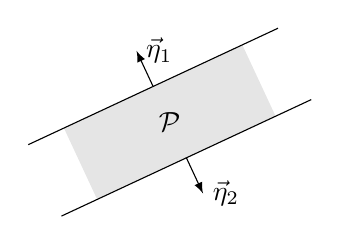
\begin{tikzpicture}
    \def\ang{25}
    \def\vecmag{.5}
    \node at (0,0) {} coordinate(p1) ++(\ang:2.5) coordinate(p2) ++(\ang-90:1.) coordinate(p3) ++(\ang-180:2.5) coordinate(p4);
    \path[fill=gray!20] (p1) -- (p2) -- (p3) -- (p4);
    \node at (barycentric cs:p1=1,p2=1,p3=1,p4=1) {$\mathcal{P}$};

    \path (p1) -- (p2) coordinate[pos=-0.2](a1l) coordinate[pos=1.2](a1r) coordinate[pos=0.5](m12);
    \draw[-latex] (a1l) -- (m12) -- ([turn] 90:0.5) node[right]{$\vec{\eta}_1$};
    \draw  (m12) -- (a1r);

    \path (p3) -- (p4) coordinate[pos=-0.2](a3l) coordinate[pos=1.2](a3r) coordinate[pos=0.5](m34);
    \draw[-latex] (a3l) -- (m34) -- ([turn] 90:0.5) node[right]{$\vec{\eta}_2$};
    \draw  (m34) -- (a3r);
  \end{tikzpicture}
  \caption{Two constraints with $\vecangle{\vec{\eta}_{1}}{\vec{\eta}_{2}}=180^{o}$.}\label{fig:parallel_only_one_active}
\end{figure}

Yet another example, are when the constraints form a convex polyhedron.
We present a minimal example of polyhedron in Fig.~\ref{fig:triangle_inequality}, a triangle in $\R^{2}$ formed by $3$ inequality constraints.
In this case, there will always be at least $2$ active constraints.
\begin{figure}[h]
  \centering
  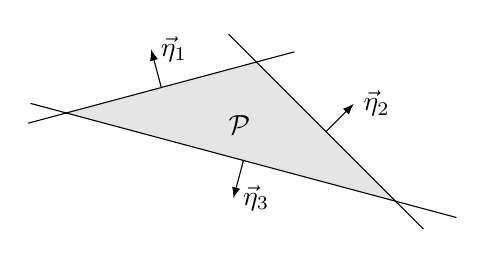
\begin{tikzpicture}
    \node at (0,0) {} coordinate(p1) ++(15:2.5) coordinate(p2) ++(-45:2.5) coordinate(p3) ++ (-195:4.0) coordinate(p4);
    \path[fill=gray!20] (p1) -- (p2) -- (p3);
    \node at (barycentric cs:p1=1,p2=1,p3=1) {$\mathcal{P}$};

    \foreach \X [count=\Y] in {2,...,4}
    {
      \path (p\Y) -- (p\X) coordinate[pos=-0.2](a\Y{}l) coordinate[pos=1.2](a\Y{}r) coordinate[pos=0.5](m\Y\X);
      \draw[-latex] (a\Y{}l) -- (m\Y\X) -- ([turn]90:.5) node[right]{$\vec{\eta}_\Y$};
      \draw (m\Y\X) -- (a\Y{}r);
    }
  \end{tikzpicture}
  \caption{A $3$-sided polyhedron.}\label{fig:triangle_inequality}
\end{figure}

Since we suppose there are at most the number of constraints as dimensions, it is not possible to create polyhedrons.

\section{Impact on negotiation equations}\label{sec:impact-local-problem}
We can try to apply the same logic used in \S\ref{sec:analysis-negotiation}, by substituting~\eqref{eq:lambdafuntheta} into~\eqref{eq:projectedSubgradient_lambda_reprise} and vice-versa, and compare with the results in \S\ref{sec:analysis-negotiation}.
In this attempt, we can fully contemplate how the relaxation of the assumptions increases the problem's complexity.

The first difficulty is already on the projected subgradient method, which due to the set
$\set{S}$ being intersection of halfplanes, does not have a straightforward solution as in the equality constraint case~\eqref{eq:example_projectedSubgradient_lambda_reprise}. The solution is found by applying the definition of the euclidean projection, which is by itself a \qp{} problem

\begin{equation}
  \Proj^{\set{X}}(\vec{x}_{0})=
  \argmin\limits_{\vec{x}}
  \left\{
    \begin{matrix}
      \minimize\limits_{\vec{x}} &
                                   \norm{\vec{x}-\vec{x}_{0}}^{2}\\
      \mathrm{subject~ to} & \vec{x}\in\set{X}\\
    \end{matrix}
  \right\},
\end{equation}
which translates to the problem
\begin{equation}
  \label{eq:projected_subgradient_qp}
  \Proj^{\set{S}}(\vec{\theta}[k]\p+\rho\p\vec{\lambda}[k]\p)=
  \argmin\limits_{\vec{x}}
  \left\{
    \begin{matrix}
      \minimize\limits_{\vec{U}[k]} &
                                      \norm{\vec{x}-\vec{\theta}[k]\p+\rho\p\vec{\lambda}[k]\p}\\
      \mathrm{subject~ to} & I_{c}^{M}\vec{x}\preceq \vec{U}_{\max}:\vec{\mu}\\
    \end{matrix}
  \right\},
\end{equation}
with corresponding dual variable $\vec{\mu}$.
For notation sake we use $\vec{x}_{0}=\vec{\theta}[k]\p+\rho\p\vec{\lambda}[k]\p$.

The problem is solved similarly to how we made in \S\ref{sec:impact-local-problem}.
Skipping some steps (calculating lagrangians and optimizing for the dual variables) we will find that the solution of $\vec{\mu}$ has the same form that~\eqref{eq:lambdafuntheta}.
However, we need to change $\bar{\Gamma}_{i}$ for $I_{c}^{M}$, $H_{i}$ for $I$, and $\vec{f}_{i}$ for $-(\vec{\theta}[k]\p+\rho\p\vec{\lambda}[k]\p)$.
And the partitions are defined by the active and inactive constraints in $I_{c}^{M}\vec{x}_{0}\preceq \vec{U}_{\max}$.

Substituting the solution of the dual variables into the lagrangian, and making the gradient vanish, will also result in a \pwa{} function with at most $2^{c}$ different modes (${\card{\elem[*,1]{I_{c}^{M}}}=c}$):
\begin{equation}
  \label{eq:projection_result_zones}
  \begin{aligned}
    \vec{\theta}[k]\pplusone=
    \begin{cases}
      \vec{x}_{0}+
      {I_{c}^{M}}^{(0)}\left[-P_{\vec{\mu}}^{(0)}\vec{U}_{max}+\vec{s}_{\vec{\mu}}^{(0)}[k]\right],&\text{if}\ \vec{x}_{0}\in\set{R}_{\vec{\mu}}^{0}\\
      \qquad\quad \vdots&\qquad\quad \vdots\\
      \vec{x}_{0},&\text{if}\ \vec{x}_{0}\in\set{R}_{\vec{\mu}}^{2^{c}-1}\\
    \end{cases}
  \end{aligned},
\end{equation}
similarly with non-overlapping regions ${\set{R}_{\vec{\mu}}^{n}=\setbuild{\vec{x}}{G_{\vec{\mu}}^{n}[k]\vec{x} \preceq \vec{U}_{\max}^{n}[k]}}$\footnote{Also not defined in this work} which partition the space of $\vec{x}_{0}$.
The non-zero elements (coded by $0$ digits in the binary representation of $(n)$) of $P_{\vec{\mu}}^{(n)}$ are ${({I_{c}^{M}}^{(n)}{{I_{c}^{M}}^{(n)}}\T)}^{-1}$, and those of $\vec{s}_{\vec{\mu}}^{(n)}[k]$ are ${{({I_{c}^{M}}^{(n)}{{I_{c}^{M}}^{(n)}}\T)}^{-1}{I_{c}^{M}}^{(n)}\vec{x}_{0}}$, ${I_{c}^{M}}^{(n)}$ is constructed by keeping/removing the constraints as coded by index $(n)$.

Observe that when all constraints are inactive ($n=0$), the solution is the same as in the equality case~\eqref{eq:euclidean_projection_equality_solution} ($\card{I_{c}^{M}}=c\times Mc$).
And when all constraints are active ($n=2^{c}-1$), the solution is the same as the unconstrained solution, since $\vec{\mu}=\0$ (see Remark~\ref{rem:sparse_solutions}).

So, we can conclude that the next value $\thetaik\pplusone$ depends on where $\vec{\theta}[k]\p+\rho\p\vec{\lambda}[k]\p$ will lie, giving at least $2^{c}$ possibilities.
In turn, $\vec{\theta}[k]\p+\rho\p\vec{\lambda}[k]\p$ depends on the values of each $\lambdaik$, which conversely can have $2^{\nineq}$ different modes each.

As in \S\ref{sec:analysis-negotiation}, when substituting the equations one in another gave us expressions of \dt{} systems, similarly here if we substitute the results for $\lambdaik$ in~\eqref{eq:projection_result_zones} we will have a switched \dt{} systems.
One with constant (in the same mode) input for $\thetaik$, and conversely a switched homogenous system for the dynamics of $\lambdaik$.

If we develop the calculations we can estimate an upper bound on the number of total different permutations $\bar{\epsilon}$, which totals to
\begin{equation}
  \label{eq:1}
  \bar{\epsilon}=\overbrace{2^{c}}^{\text{regions in projection}}\times \underbrace{2^{\nineq}\times \dots \times 2^{{\nineq}}}_{M\times \text{regions in each }\lambdai }=2^{c+M\nineq}.
\end{equation}

\begin{remark}
  Probably some of those permutations may not be possible, but still we have exponential growth on the number of modes of the switched systems.
  The exact calculation for the regions is not the scope of this work.
\end{remark}

The case for scarce systems seen in the last chapter, settles the solution of the projection to the case $(0)$, where $\vec{\theta}[k]\p+\rho\p\vec{\lambda}[k]\p$ is projected onto the intersection of all halfspaces.
And due to another assumption (that $\bar{\Gamma}_{i}\optuncUik\succ \thetaik, \forall i\in\set{M}, \forall k$), we fix all $\lambdai$ to the first solution in~\eqref{eq:lambdafuntheta}.
This consecutive choices of assumptions reduces the total number of switching modes to exactly one, presented by equations~\eqref{eq:negotiation_equation_substituting_organizing_matrix_lambda} and~\eqref{eq:negotiation_equation_substituting_organizing_matrix_theta}, reproduced here.

\begin{equation}
  \label{eq:negotiation_equation_substituting_organizing_matrix_lambda_reprise}
  \tag{\ref*{eq:negotiation_equation_substituting_organizing_matrix_lambda}}
  \vec{\lambda}\pplusone=\mathcal{A}_{\lambda}\vec{\lambda}\p,
\end{equation}
\begin{equation}
  \label{eq:negotiation_equation_substituting_organizing_matrix_theta_reprise}
  \tag{\ref*{eq:negotiation_equation_substituting_organizing_matrix_theta}}
  \vec{\theta}\pplusone=\mathcal{A}_{\theta}\vec{\theta}\p+\mathcal{\vec{B}}_{\theta}[k]
\end{equation}

If we concatenate the binary representations of the modes of the projection and of each local problem, we will have a number with $c+M\nineq$ digits.
And thus, the solutions in ~\eqref{eq:negotiation_equation_substituting_organizing_matrix_lambda} and~\eqref{eq:negotiation_equation_substituting_organizing_matrix_theta} can be seen as an specific case of the following solutions for the $0$-th modes:
\begin{equation}
  \label{eq:negotiation_equation_substituting_organizing_matrix_lambda_switched}
  \vec{\lambda}[k]\pplusone=
  \begin{cases}
    \mathcal{A}_{\lambda}^{0}\vec{\lambda}[k]\p,&\text{if}\ \vec{\theta} \in \set{R}_{\vec{\lambda}}^{0}\\
    \quad\vdots&\quad\vdots\\
    \mathcal{A}_{\lambda}^{N_{\vec{\lambda}}}\vec{\lambda}[k]\p,&\text{if}\ \vec{\theta}\in\set{R}_{\vec{\lambda}}^{0}\\
  \end{cases}
\end{equation}
\begin{equation}
  \label{eq:negotiation_equation_substituting_organizing_matrix_theta_switched}
  \vec{\theta}[k]\pplusone=
  \begin{cases}
    \mathcal{A}_{\theta}^{0}\vec{\theta}[k]\p+\mathcal{\vec{B}}_{\theta}^{0}[k],&\text{if}\ \vec{\theta}\in\set{R}_{\vec{\theta}}^{0}\\
    \qquad\quad \vdots&\quad \vdots\\
    \mathcal{A}_{\theta}^{N_{\vec{\theta}}}\vec{\theta}[k]\p+\mathcal{\vec{B}}_{\theta}^{N_{\vec{\theta}}}[k],&\text{if}\ \vec{\theta}\in\set{R}_{\vec{\theta}}^{N_{\vec{\theta}}}\\
  \end{cases}
\end{equation}

where $N_{\vec{\lambda}}=N_{\vec{\theta}}=2^{c+M\nineq}-1$.
The non-overlapping regions described by tuples
 ${\set{R}_{\vec{\lambda}}^{n}=\setbuild{\vec{x}}{G_{\vec{\lambda}}^{n}[k]\vec{\theta}[k]\p \preceq \vec{b}_{\vec{\lambda}}^{n}[k]}}$, and
 ${\set{R}_{\vec{\theta}}^{n}=\setbuild{\vec{x}}{G_{\vec{\theta}}^{n}[k]\vec{\theta}[k]\p \preceq \vec{b}_{\vec{\theta}}^{n}[k]}}$
coincide, and are formed by the superposition of the regions $\set{R}_{\lambdai}^{n}$ in~\eqref{eq:projection_result_zones} and $\set{R}_{\vec{\mu}}^{n}$ in~\eqref{eq:lambdafuntheta}.
We highlight again that not necessarily all permutations are possible (some regions are empty).

Observe that in some cases, it is straightforward to define the values of the matrices in~\eqref{eq:negotiation_equation_substituting_organizing_matrix_lambda_switched} and~\eqref{eq:negotiation_equation_substituting_organizing_matrix_theta_switched}.
The $0$-th case, as mentioned, is the same we found in the last chapter, giving
$\mathcal{A}_{\vec{\lambda}}^{0}=\mathcal{A}_{\vec{\lambda}}$,
$\mathcal{A}_{\vec{\theta}}^{0}=\mathcal{A}_{\vec{\theta}}$, and
$\vec{B}_{\vec{\theta}}^{0}[k]=\vec{B}_{\vec{\theta}}[k]$.
Similarly for the $N_{\vec{\theta}}$-th case where all the constraints of all systems are active (implying all $\lambdai=\0$), and the projection of $\vec{\theta}[k]\p+\rho\p\vec{\lambda}[k]\p$ is itself, yielding
$\mathcal{A}_{\vec{\lambda}}^{N_{\vec{\lambda}}}=0_{\card{\vec{\lambdai}}}$,
$\mathcal{A}_{\vec{\theta}}^{N_{\vec{\theta}}}=I_{\card{\vec{\thetai}}}$, and
$\vec{B}_{\vec{\theta}}^{N_{\vec{\theta}}}[k]=\0$.
The $N_{\vec{\theta}}$-th case is trivial since it means the optimal value was already found, $\vec{\theta}[k]\pplusone=\vec{\theta}[k]\p$.

Applying the attack ~\eqref{eq:linear_attack}, using cheating matrices $T_{i}$ we can have simular results

\begin{equation}
  \label{eq:negotiation_equation_substituting_organizing_matrix_lambda_switched_cheating}
  \tilde{\vec{\lambda}}[k]\pplusone=
  \begin{cases}
    \tilde{\mathcal{A}}_{\lambda}^{0}\tilde{\vec{\lambda}}[k]\p,&\text{if}\ \vec{x}_{0}\in\set{R}_{\vec{\lambda}}^{0}\\
    \quad\vdots&\quad\vdots\\
    \tilde{\mathcal{A}}_{\lambda}^{N_{\vec{\lambda}}}\tilde{\vec{\lambda}}[k]\p,&\text{if}\ \vec{x}_{0}\in\set{R}_{\vec{\lambda}}^{N_{\vec{\lambda}}}\\
  \end{cases}
\end{equation}
\begin{equation}
  \label{eq:negotiation_equation_substituting_organizing_matrix_theta_switched_cheating}
  \vec{\theta}[k]\pplusone=
  \begin{cases}
    \tilde{\mathcal{A}}_{\theta}^{0}\vec{\theta}[k]\p+\mathcal{\tilde{\vec{B}}}_{\theta}^{0}[k],&\text{if}\ \vec{\theta}\in\set{R}_{\vec{\theta}}^{0}\\
    \qquad\quad \vdots&\quad \vdots\\
    \tilde{\mathcal{A}}_{\theta}^{N_{\vec{\theta}}}\vec{\theta}[k]\p+\mathcal{\tilde{\vec{B}}}_{\theta}^{N_{\vec{\theta}}}[k],&\text{if}\ \vec{\theta}\in\set{R}_{\vec{\theta}}^{N_{\vec{\theta}}}\\
  \end{cases}
\end{equation}
One can observe that since we multiply $\lambdai$ by $T_{i}[k]$, we do not change the partition of the spaces.
We can similarly see that
$\tilde{\mathcal{A}}_{\vec{\lambda}}^{0}=\tilde{\mathcal{A}}_{\vec{\lambda}}$,
$\tilde{\mathcal{A}}_{\vec{\theta}}^{0}=\tilde{\mathcal{A}}_{\vec{\theta}}$,
$\tilde{\vec{B}}_{\vec{\theta}}^{0}[k]=\tilde{\vec{B}}_{\vec{\theta}}[k]$, and all analysis made in the last chapter also holds for this mode.

\begin{remark}\label{rem:cheat_satisfied_problem}
  One interesting fact we can observe is, for cases where the corresponding $\lambdai$ is already $\0$, the multiplication of $T_{i}$ will not affect its value.
  A satisfied agent, i.e., an agent whose local problem has same solution than its unconstrained version, has no motive to get more resources, since the allocated resources will satisfy its needs.
  So, in the most extreme case, specifically the $N_{\vec{\theta}}$-th mode, we see that
  even if all agents cheat at the same time, there is no impact of the cheat, since they are all satisfied, $\lambdai=\0\ \forall i \in \set{M}$, resulting in
  $\tilde{\mathcal{A}}_{\vec{\lambda}}^{N_{\vec{\lambda}}}=\mathcal{A}_{\vec{\lambda}}^{N_{\vec{\lambda}}}$,
  $\tilde{\mathcal{A}}_{\vec{\theta}}^{N_{\vec{\theta}}}=\mathcal{A}_{\vec{\theta}}^{N_{\vec{\theta}}}$, and
  $\tilde{\vec{B}}_{\vec{\theta}}^{N_{\vec{\theta}}}[k]=\vec{B}_{\vec{\theta}}^{N_{\vec{\theta}}}[k]$.
\end{remark}

We could analyze stability in a case-by-case fashion, seeing what constraints are active/inactive for which agent and how the cheating matrices influence the stability.
But due to the extension of the analysis (exponential number of cases) we skip it for brevity's sake, and will use a single example, different from the trivial solution, to illustrate how it could be done.

Denoting as the zone (or region) $n$, or the $n$-zone, the non-overlapping polytopes defined by ${\set{R}^{n}=\setbuild{\vec{x}}{G_{\vec{\theta}}^{n}[k]\vec{x} \preceq \vec{b}_{\vec{\theta}}^{n}[k]}}$, we retake our $2$-constraints example in Fig.~\ref{fig:constraints_partition_theta}.
Since there are $2$ constraints, we set for example $c=1$ and $\predhorz=2$, then we have at most $4$ different modes on the solution for $\lambdaicheat$:
\begin{equation}
  \lambdaicheat[k]=
  \begin{cases}
    -\Plinineqtilde      \thetaik-\sikineqtilde      ,&\text{if }\thetaik\in\set{R}^{0}\\
    -\Plinineqtilde[i][1]\thetaik-\sikineqtilde[i][1],&\text{if }\thetaik\in\set{R}^{1}\\
    -\Plinineqtilde[i][2]\thetaik-\sikineqtilde[i][2],&\text{if }\thetaik\in\set{R}^{2}\\
    -\Plinineqtilde[i][3]\thetaik-\sikineqtilde[i][3],&\text{if }\thetaik\in\set{R}^{3}\\
  \end{cases}\label{eq:1}
\end{equation}
where
\begin{align}
  \Plinineqtilde&=T_{i}{{(\linearcoefiineqnonzero)}^{-1}}&&=&&T_{i}{(\linearcoefi)}^{-1}\\
  \Plinineqtilde[i][1]&=T_{i} \left[
                        \begin{matrix}
                          {{(\linearcoefiineqnonzero[1,*])}^{-1}}&0\\
                          0&0
                        \end{matrix}
                             \right]&&=&& \left[
                                          \begin{matrix}
                                            \elem[1,1]{T_{i}}{{(\linearcoefiineqnonzero[1,*])}^{-1}}&0\\
                                            \elem[2,1]{T_{i}}{{(\linearcoefiineqnonzero[1,*])}^{-1}}&0\\
                                          \end{matrix}
  \right]\\
  \Plinineqtilde[i][2]&=T_{i} \left[
                        \begin{matrix}
                          0&0\\
                          0&{{(\linearcoefiineqnonzero[2,*])}^{-1}}\\
                        \end{matrix}
  \right]&&=&& \left[
               \begin{matrix}
                 0&\elem[1,2]{T_{i}}{{(\linearcoefiineqnonzero[2,*])}^{-1}}\\
                 0&\elem[2,2]{T_{i}}{{(\linearcoefiineqnonzero[2,*])}^{-1}}\\
               \end{matrix}
  \right]
  \\
  \Plinineqtilde[i][3]&=T_{i}
                        \left[
                        \begin{matrix}
                          0&0\\
                          0&0
                        \end{matrix}
                             \right]&&=&&\left[
                                          \begin{matrix}
                                            0&0\\
                                            0&0
                                          \end{matrix}
                                               \right]
\end{align}
\begin{align}
  \sikineqtilde[i][0]&=&&T_{i}\sikineq[i][0]&&=&&T_{i}{(\linearcoefi)}^{-1}\bar{\Gamma}_{i}H_{i}^{-1}\vec{f}_{i}[k]\\
  \sikineqtilde[i][1]&=&&T_{i} \sikineq[i][1]&&=&& \left[
                                                   \begin{matrix}
                                                     \elem[1,1]{T_{i}}{{(\linearcoefiineqnonzero[1,*])}^{-1}}\elem[1,*]{\bar{\Gamma}_{i}}H_{i}^{-1}\vec{f}_{i}[k]\\
                                                     \elem[2,1]{T_{i}}{{(\linearcoefiineqnonzero[1,*])}^{-1}}\elem[1,*]{\bar{\Gamma}_{i}}H_{i}^{-1}\vec{f}_{i}[k]\\
                                                   \end{matrix}
  \right]\\
  \sikineqtilde[i][2]&=&&T_{i} \sikineq[i][2]&&=&& \left[
                                                   \begin{matrix}
                                                     \elem[1,2]{T_{i}}{{(\linearcoefiineqnonzero[2,*])}^{-1}}\elem[2,*]{\bar{\Gamma}_{i}}H_{i}^{-1}\vec{f}_{i}[k]\\
                                                     \elem[2,2]{T_{i}}{{(\linearcoefiineqnonzero[2,*])}^{-1}}\elem[2,*]{\bar{\Gamma}_{i}}H_{i}^{-1}\vec{f}_{i}[k]\\
                                                   \end{matrix}
  \right]
  \\
  \sikineqtilde[i][3]&=&&T_{i}\sikineq[i][3] &&=&&\left[
                                                   \begin{matrix}
                                                     0\\ 0
                                                   \end{matrix}
  \right]
\end{align}
with
\begin{align}
  \sikineq[i][0]&={{(\linearcoefiineqnonzero)}^{-1}}\elem[*,*]{\bar{\Gamma}_{i}}H_{i}^{-1}\vec{f}_{i}[k]\\
  \sikineq[i][1]&= \left[
                  \begin{matrix}
                    {{(\linearcoefiineqnonzero[1,*])}^{-1}}\elem[1,*]{\bar{\Gamma}_{i}}H_{i}^{-1}\vec{f}_{i}[k]\\
                    0
                  \end{matrix}
  \right]\\
  \sikineq[i][2]&=\left[
                  \begin{matrix}
                    0\\
                    {{(\linearcoefiineqnonzero[2,*])}^{-1}}\elem[2,*]{\bar{\Gamma}_{i}}H_{i}^{-1}\vec{f}_{i}[k]\\
                  \end{matrix}
  \right]\\
  \sikineq[i][3]&= \left[
                  \begin{matrix}
                    0\\
                    0
                  \end{matrix}
  \right]
\end{align}

One can observe that for zones $1$ and $2$, when the agent attacks, the non-zero elements of $\Plinineq[i][n]$ and $\sikineq[i][n]$, influences the other elements using the columns of $T_{i}$ equivalent to the inactive constraints.
For example in zone $1$, $\elem[1,1]{T_{i}}$ and $\elem[2,1]{T_{i}}$ are used, and for zone $2$, $\elem[1,2]{T_{i}}$ and $\elem[2,2]{T_{i}}$.
\begin{remark}
  Observe that if $T_{i}$ is diagonal, there is no injection of ``inactive elements'' into an ``active elements''.
\end{remark}

So, instead of always propagating to the negotiation all the matrix $T_{i}$, as in the case of the last chapter, only the columns related to the inactive constraints are propagated.

If we have $M=2$ subsystems, one in the $1$-zone and other in the $2$-zone (let us called them agents I and II) and we suppose the solution of the projection is in its $0$-zone, i.e., ${G_{\vec{\mu}}^{0}[k](\vec{\theta}[k]\p+\rho\p\vec{\lambda}[k]\p) \preceq \vec{U}_{\max}^{0}[k]}$, we code the permutation as
\begin{equation}
  \underbrace{00}_{\text{projection's zone}}\overbrace{01}^{\text{agent I`s zone}}\underbrace{10}_{\text{agent II's zone}} = 000110_{(2)}=6_{(10)}.
\end{equation}

Applying the projection, we will have the same solution~\eqref{eq:euclidean_projection_equality_solution}, reprised here
\begin{equation}
  \label{eq:euclidean_projection_equality_solution_reprise}
  \tag{\ref*{eq:euclidean_projection_equality_solution}}
  \vec{\theta}\pplusone=\vec{\theta}\p+\rho\p\vec{\lambda}\p+{I_{c}^M}\T/({I_{c}^M} {I_{c}^M}\T)\left({I_{c}^M}(\vec{\theta}\p-\rho\p\vec{\lambda}\p) -\vec{U}_{\max}\right),
\end{equation}
which can be rewritten for each $\thetai$ as
\begin{equation}
  \thetai\pplusone= \thetai\p + \frac{1}{M}\left(\sum_{j\in\set{M}}\vec{\theta}_{j}\p-\vec{U}_{\max}\right) + \rho\p\left(\vec{\lambda}\p-\frac{1}{M}\sum_{j\in\set{M}}\vec{\lambda}_j\p\right)
\end{equation}
and substituting the $\lambdai$ by $\lambdaicheat$:
\begin{align}
  \vec{\theta}_{i}\pplusone=
  \vec{\theta}_{i}\p+
  \frac{1}{M}\left(\sum_{j\in\set{M}}\vec{\theta}_{j}\p-\vec{U}_{\max}\right)&
                                                                     + \rho\p\left(
                                                                     -\Plinineqtilde[i][n(i)]\thetai\p-\sikineqtilde[i][n(i)]
                                                                     \right) \notag\\
                                                                   &-\frac{\rho\p}{M}\sum_{j\in\set{M}}\left(
                                                                     -\Plinineqtilde[j][n(j)]\vec{\theta}_{j}\p-\sikineqtilde[j][n(j)]
                                                                     \right)
\end{align}
where $n(i)$ indicates the coding of the zone of agent $i$.

Grouping the terms we have
\begin{align}
  \thetai\pplusone=\thetai\p+\rho\p\left(-\Plinineqtilde[i][n(i)]\thetai\p+\frac{1}{M}\sum_{j\in\set{M}}\Plinineqtilde[j][n(j)]\vec{\theta}_{j}\p\right)+\frac{1}{M}\left(\sum_{j\in\set{M}}\vec{\theta}_{j}\p\right)\\+\rho\p\left(-\sik+\frac{1}{M}\sum_{j\in\set{M}}\vec{s}_{j}[k]\right) -\frac{\vec{U}_{\max}}{M}
\end{align}
resulting in
\begin{equation}
  \vec{\theta}\pplusone=\tilde{\mathcal{A}}_{\theta}^{(6)}\vec{\theta}\p+\tilde{\mathcal{\vec{B}}}_{\theta}^{(6)}[k]
\end{equation}
where
\begin{equation}
  \tilde{\mathcal{A}}_{\theta}^{(6)}=\left[
    \begin{matrix}
      2I-\frac{1}{2}\rho\p \Plinineqtilde[I][1] & I+\frac{1}{2}\rho\p \Plinineqtilde[II][2]\\
      I+\frac{1}{2}\rho\p \Plinineqtilde[I][1] & 2I-\frac{1}{2}\rho\p \Plinineqtilde[II][2]\
    \end{matrix}
  \right]
\end{equation}
\begin{equation}
  \tilde{\mathcal{\vec{B}}}_{\theta}^{(6)}[k]=\left[
    \begin{matrix}
      -\frac{1}{2}\rho\p \sikineqtilde[I][1]+\frac{1}{2}\rho\p \sikineqtilde[II][2]-\frac{\vec{U}_{\max}}{2}\\
      \frac{1}{2}\rho\p \sikineqtilde[I][1]-\frac{1}{2}\rho\p \sikineqtilde[II][2]-\frac{\vec{U}_{\max}}{2}
    \end{matrix}
  \right]
\end{equation}

And we can see that, as expected, the columns of $T_{i}$ are propagated to $\mathcal{A}_{\vec{\theta}}$, and may change its dynamics.
We could do the same for the dynamics of $\lambdai$, but we let this for the reader.

For the overall system dynamics we may use any tools for analysis of hybrid/ switched systems~\cite{BorrelliEtAl2017}.

\begin{remark}
  Observe that since the matrices $\mathcal{A}_{\vec{\theta}}^{n}$ and $\mathcal{A}_{\vec{\lambda}}^{n}$ may be sparse, the eigenvalue analysis to indicate stability of the mode is accomplished by keeping only the non-zero corresponding blocks.
\end{remark}

As we see, the relaxation of the assumption makes the problem exponentially more complicated.
In the next section we will discuss ways to adapt the detection and mitigation strategies to overcome the complexity presented.

\section{Adapting detection and mitigation methods}\label{sec:detection-mitigation}

We propose to use a similar strategy to the one used in the last chapter.
However, some difficulties arise.
We do not have one tuple $(\Plin,\sik)$ for each subsystem, but we have $2^{\predhorz c}$ different tuples.

Here follow proposals on how to counter the difficulties.

\subsection{Mitigation}\label{sec:mitigation_ineq}
We begin by the end, with the proposal for the mitigation because the proposal follows a straightforward logic and impacts the proposal for the detection, simplifying its solution.

We still want to mitigate the effects of the attack by reconstructing $\lambdai$.
So, if we assume we can somehow estimate the inverse of the cheating matrix $T_{i}$, which we still assume is invertible (See~\eqref{eq:T_is_invertible}), we can easily try to reconstruct $\lambdai$ by applying
\begin{equation}
  \label{eq:lambda_reconstruction}
  \lambdaireconstructed=\Tikinvestimate \lambdaicheat.
\end{equation}

However, estimating $\Tikinvestimate$ is a bit more difficult then before.
We cannot use~\eqref{eq:estimate_T_inverse} anymore (reprised for clarity), since we do not have $\Plin$.
\begin{equation}
  \label{eq:estimate_T_inverse_reprise}
  \tag{\ref*{eq:estimate_T_inverse}}
  {\Tikinvestimate=\Plinnominal{\Plintildeestimate}^{-1}}.
\end{equation}

If we estimate any $\Plinineq[i][n]$, not necessarily we can invert it.
As seen in \S\ref{sec:impact-local-problem}, almost all $\Plinineq[i][n]$ are sparse with rows and columns equal to zero, thus singular.
The only one that is invertible is $\Plinineq$.
So if we can estimate $\Plinineqtilde$ and we have a nominal $\Plinineqnominal$ (probably estimated the same way during an attack-free trial), we can estimate $\Tikinvestimate$ similarly:
\begin{equation}
  \label{eq:estimate_T_inverse_ineq}
  {\Tikinvestimate=\Plinineqnominal{\Plinineqtildeestimate}^{-1}}.
\end{equation}

So, we assume that $\Plinineq$ exists and that is possible to estimate it.

The necessary condition for existence of the $0$-th region ($0$-zone) is that we can choose $\thetai$ such the constraints $\inequalityfunction$ are inactive for the unconstrained solution $\optuncUik$.
Since we can only choose $\thetai$ that respects $\dom J_{i}$, to assure feasibility, we assume the unconstrained solution $\optuncU$ and $\optuncUik$ lie inside
the respective constraint sets
\begin{align}
  \optuncU\in\set{U}\\
  \optuncUik\in\set{U}_{i}.
\end{align}

\newcommand{\thetairestricted}{\overset{\rotatebox{90}{r}}{\thetai}}

We call \emph{artificial scarcity} the method of forcing the constraints to be inactive.
And supposing there is a value $\thetairestricted$ that deactivates all constraints, we call it the \emph{artificial scarcity point}.

So, if we can generate points in a ball ($\set{B}(\vec{x}_{c},r)=\setbuild{\vec{x}}{\norm{\vec{x}-\vec{x}_{c}}\leq r}$) around $\thetairestricted$\note{choose a better notation, please} (See Fig.~\ref{fig:ball_around_theta_restricted}), we can use the same method of supervision of communication of the coordinator and agents used in the last chapter to estimate $\Plinineq$.

However, one complication arises when choosing the size of the ball around $\thetairestricted$, since it may traverse one of the frontiers of the polytope and generate points corresponding to other modes (See Fig.~\ref{fig:ball_around_theta_restricted_traversing}).

\begin{figure}[h]
  \centering
  \begin{subfigure}{0.4\textwidth}
    \centering
    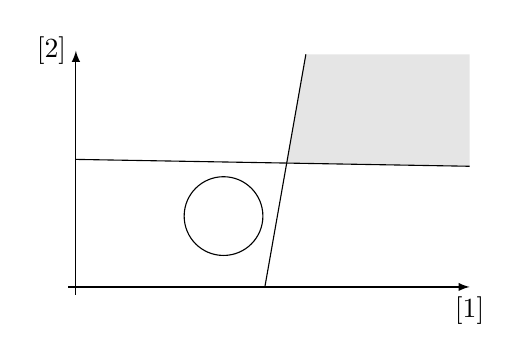
\begin{tikzpicture}
      \def\height{3}
      \def\length{5}
      \node at (0,0) {} coordinate (p0)  ++(0:\length*2.4/5) coordinate (p1) ;
      \node at (0,0) {} ++(90:\height*2.7/5) coordinate (p2) ;

      \draw[black] (p2) ++(-1:5) coordinate (p3);
      \draw[black] (p1) ++(80:3) coordinate (p4);
      \coordinate (p6) at (p3|-p4);

      \coordinate (p5) at (intersection cs:first line={(p2)--(p3)}, second line={(p1)--(p4)});
      \path[fill=gray!20] (p6) -- (p4) -- (p5) -- (p3);
      \draw[black] (p2) -- (p3);
      \draw[black] (p1) -- (p4);

      \draw[-latex] (0,-.1) - - (0,\height) node[left]{$\elem[2]{\thetai}$};
      \draw[-latex] (-.1,0) - - (\length,0) node[below]{$\elem[1]{\thetai}$};

      \node[draw,circle,minimum width=1cm] at (\length*.375,\height*0.3) {$\thetairestricted$};
    \end{tikzpicture}
    \caption{Ball $\set{B}(\thetairestricted,r)$.}\label{fig:ball_around_theta_restricted}
  \end{subfigure}
  \hfill
  \begin{subfigure}{0.4\textwidth}
    \centering
    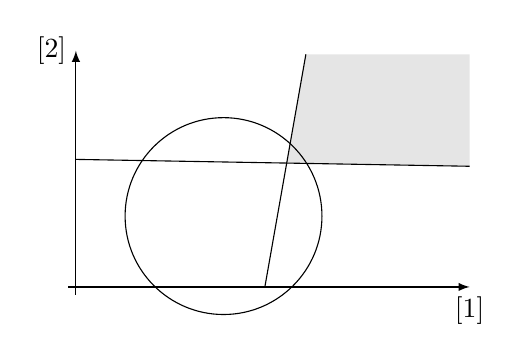
\begin{tikzpicture}
      \def\height{3}
      \def\length{5}
      \node at (0,0) {} coordinate (p0)  ++(0:\length*2.4/5) coordinate (p1) ;
      \node at (0,0) {} ++(90:\height*2.7/5) coordinate (p2) ;

      \draw[black] (p2) ++(-1:5) coordinate (p3);
      \draw[black] (p1) ++(80:3) coordinate (p4);
      \coordinate (p6) at (p3|-p4);

      \coordinate (p5) at (intersection cs:first line={(p2)--(p3)}, second line={(p1)--(p4)});
      \path[fill=gray!20] (p6) -- (p4) -- (p5) -- (p3);
      \draw[black] (p2) -- (p3);
      \draw[black] (p1) -- (p4);

      \draw[-latex] (0,-.1) - - (0,\height) node[left]{$\elem[2]{\thetai}$};
      \draw[-latex] (-.1,0) - - (\length,0) node[below]{$\elem[1]{\thetai}$};

      \node[draw,circle,minimum width=2.5cm] at (\length*.375,\height*0.3) {$\thetairestricted$};
    \end{tikzpicture}
    \caption{Ball $\set{B}(\thetairestricted,r)$ traversing zones.}\label{fig:ball_around_theta_restricted_traversing}
  \end{subfigure}
  \caption{Effects of different radii $r$ when generating points close to $\thetairestricted$.}
\end{figure}

Therefore, we need an estimation method that can also classify simultaneously the points, indicating to which zone they correspond.
Then, we take only the parameters that interest us, that is $\Plinineq$.

In \S\ref{sec:cons-about-mult}, we will discuss estimation methods and we describe the proposed method to solve this problem.

\subsection{Detection}\label{sec:detection_ineq}
For the detection we can use the same logic presented in the last chapter.

As we can observe in~\eqref{eq:lambdafuntheta}, the affine parts $\Plinineq[i][n]$ are time-invariant.
So, if we estimate the affine parts $\Plinineqtildeestimate[i][n]$, we can detect an attack when there is any difference between the estimated and nominal values $\Plinineqnominal[i][n]$.
We can compare the estimates with nominals from any non-zero mode\footnote{$2^{Nc}$-zones have empty elements, which do not change when the cheating matrices are applied (\S\ref{sec:impact-local-problem}).}.
However, since we are going to use $\Plinineqtildeestimate$ for the mitigation part, we can also use it for the detection.

Analogously, we can set an arbitrary bound $\epsilon_{\Plinineq}$, and define the error
\begin{equation}
  E_{i}^{(0)}[k] =\norm{\Plinineqtildeestimate-\Plinineqnominal}_{F},
\end{equation}
which associated with an detection function $d_{i}^{(0)}$:
\begin{equation}
  \label{eq:detection_ineq}
  d_{i}^{(0)}=\indicator{E_{i}^{(0)}[k]\geq\epsilon_{\Plinineq}},
\end{equation}
detects an attack when the corresponding bound is disrespected, i.e., $d_{i}^{(0)}=1$.

\section{About Multiple Parameter Estimation}\label{sec:cons-about-mult}
The problem of estimating affine parameters on a system with a known number of different modes is called in~\cite{LauerBloch2019} as a \emph{\pwa{} regression with fixed modes}.
The problem is formalized in a optimization problem which we adapt for our case.
To find the $\pwaestnumparam$ different parameters $\pwaestparam_{i}$ of the \pwa{} function with non-overlapping regions $\set{R}^{i}$ such $\bigcup_{i=1}^{\pwaestnumparam}\set{R}^{i}=\set{R}$, we take a set of $\pwaestinputsize$ inputs/output tuples $(\pwaestsysinput_{k},\pwaestsysoutput_{k})|_{k\in\{1:\pwaestinputsize\}}\subset\R^{\card{\pwaestsysinput}}\times\R^{\card{\pwaestsysoutput}}$ and solve

\begin{equation}
    \minimize_{\pwaestparam \in \R^{\pwaestnumparam \card{\elem[1,*]{\pwaestsysinput}}}} \frac{1}{\pwaestinputsize} \sum_{k=1}^{\pwaestinputsize} \sum_{j=1}^{\pwaestnumparam} \mathbb{1}_{g\left(\pwaestsysinput_{k}\right)=j} \norm{\norm{\pwaestsysoutput_{k}- \pwaestsysinput_{k}\pwaestparam_{j}}_{1}}.
\end{equation}
where $g:\R^{\card{\pwaestsysinput}}\to\{1:\pwaestnumparam\}$ is a linear classification function, which classifies the membership of its argument, returning the corresponding index of the region it is member of.
The definition of such function can be seen in~\cite{LauerBloch2019}.
Observe that since the output of $g$ is an integer ($\{1:\pwaestnumparam\}\subset\Z$), the problem is a \miqp{} program.
In this work we are not interested in determining the classification functions,  but just the parameters.

As commented in~\cite{LauerBloch2019}, since the program is a \miqp{} if we try to solve the problem by brute force (trying all the combinations), the complexity increases exponentially depending on the number of modes $\pwaestnumparam$ and inputs $\pwaestinputsize$.
So, some clever methods were created to exploit the problem structure, by successively solving different optimization problems for example. Some strategies are listed in~\cite{RollEtAl2004}.

The most known examples of these strategies are the methods in the \emph{partitional family}.
The methods in this family solve partition and regression problems successively.
Notable members of the family are the widely used k-means~\cite{Ferrari-TrecateEtAl2001} and k-medoids~\cite{Bishop2006} methods.

In these methods, estimates of the parameters are used to classify membership of all points, assigning a region to each input, and then, the points are used to solve different regression problems, updating the parameter estimates of their corresponding region.

Another similar method~\cite{Bishop2006}, which can also be categorized in the same family, is the \EM{} method~\cite{DempsterEtAl1977}.
The \EM{} is the method of choice in this chapter to estimate the parameters needed for the detection and mitigation phases.

We could have used any of the other methods cited, but we chose \EM{} for it not making a hard assignment of the points, but instead a soft choice based on probabilities, what we will see gives us favorable properties on convergence.

This method is not commonly used by the control community, being more frequently used in the machine learning/data mining areas.
However, an inspiring example was proposed for the estimation of switched systems in~\cite{NakadaEtAl2005}.

In the next subsection we describe the method more precisely.

\subsection{Expectation Maximization}
The main objective of the \EM{} algorithm is to find, from a set of observable data $\set{B}$, estimators of a set of parameters $\set{P}$ that maximize the log marginal likelihood of the observed data ${\ln\probability{\set{B};\set{P}}}$. The models generally have latent variables (unobservable) in a set $\set{U}$.

The problem is that maximizing ${\ln\probability{\set{B};\set{P}}}$ does not have an analytical solution.
So, the algorithm solves the optimization problem in a iterative manner.

Instead of estimating the $\set{P}$ that maximizes ${\ln\probability{\set{B};\set{P}}}$, we find estimates that maximizes the expectation of the complete-data log-likelihood $\ln\probability{\set{B},\set{U};\set{P}}$ w.r.t.
the posterior probabilities ${\probability{\set{U}|\set{B};\set{P}}}$.

Though, as we need to have $\set{P}$ to calculate the posterior probabilities, we
calculate it using a current estimates of $\set{P}$ denoted $\set{P}_{\mathrm{cur}}$.
And repeating the same strategy with the new found estimate, we can approach the estimates which maximizes the log marginal likelihood.

The successive steps of calculating the posterior probabilities (expectation) and maximizing the complete-data log-likelihood, gives it the name Expectation Maximization.
These steps provide a monotonic increase of the log-marginal likelihood at each iteration, yielding guaranteed convergence for a local maximum.

The iterative algorithm can be resumed in Algorithm~\ref{alg:em}.

\SetKwBlock{Estep}{ E step:}{}
\SetKwBlock{Mstep}{ M step:}{}
\begin{algorithm2e}[h]
  \DontPrintSemicolon%
  Initialize parameters $\set{P}_{\mathrm{new}}$\;
  \Repeat{$\set{P}_{\mathrm{cur}}$ converges}{
    $\set{P}_{\mathrm{cur}}\gets\set{P}_{\mathrm{new}}$\;
    \Estep{
      Evaluate ${\probability{\set{U}|\set{B};\set{P}_{\mathrm{cur}}}}$\;
    }
    \Mstep{
      Estimate $\set{P}_{\text{new}}$: \begin{equation}
        \label{eq:m_step}
        \set{P}_{\mathrm{new}}=\argmax_{\set{P}}\ \expectation[{\probability{\set{U}|\set{B};\set{P}_{\mathrm{cur}}}}]{\ln\probability{\set{B},\set{U};\set{P}}}
      \end{equation}
    }
}
 \caption{Expectation Maximization}\label{alg:em}
\end{algorithm2e}

\begin{remark}\label{rem:em_depends_on_initialization}
  The method has guaranteed convergence for local maxima, which depend on the initialization of the estimates of $\set{P}$~\cite{BaudryCeleux2015,GepperthPfuelb2021}.
  The choice of initial estimates is not in the scope of this work, the reader is referred to~\cite{KarlisXekalaki2003,BaudryCeleux2015}, where the authors analyze the choice for initialization.
\end{remark}

\subsection{Adapting the problem to use the method}
Since the \EM{} is a probabilistic method, we need to have a probabilistic regression model, which is not our case.
The idea is to incorporate probabilistic behavior to our model~\eqref{eq:lambdafuntheta}.

As the method will be used for all agents at every negotiation, we drop the subscript $i$ and the time dependency $[k]$, simplifying the notation.

So, we exchange our original deterministic variables $\thetai$ and $\lambdai$, for their stochastic counterparts denoted $\random{\thetai}$ and $\random{\lambdai}$.

If we watch $O$ exchanges between an agent and the coordinator, we can observe the input and response variables, identified as ${\random{\vec{\theta}}_{o}}$ and ${\random{\vec{\lambda}}_{o}}$, ${o\in\set{O}=\{1\until O\}}$.
The input and response can be organized in ${\random{\Theta},\random{\Lambda}\in\R^{c\times O}}$.
The tuple ${(\random{\Theta},\random{\Lambda})}$ is the observable data $\set{B}$.

Since each $\randomvec{\theta}_{o}$ belongs to a given region, we associate a variable $z\in\set{Z}=\{0\until Z-1\}$ which indicates the number of a zone.
We can construct then our regression model as

\begin{equation}\label{eq:linear_cheating_random}
  \randomvec{\lambda}_{o}=
  \begin{cases}
    -\tilde{P}^{0}\randomvec{\theta}_{o}-\tilde{\vec{s}}^{0},&\text{if in zone } 0\\
    \qquad\quad \vdots&\qquad\quad \vdots\\
    -\tilde{P}^{Z-1}\randomvec{\theta}_{o}-\tilde{\vec{s}}^{Z},&\text{if in zone } Z-1\\
  \end{cases}.
\end{equation}

In~\cite{FariaSoromenho2010}, a somehow similar model is called \emph{mixture of linear regressions}, but since we are using \pwa{} functions, which have linear and constant terms, we will called the model \emph{mixture of affine regressions}.

Since we don't known the partitions or the belonging of each observed point, we associate the index $z$ of each observation ${(\randomvec{\lambda}_{o}, \randomvec{\theta}_{o})}$ to a latent random variable ${\random{z}_{o}}$.
We can organize the $\random{z}_{o}$ variables into ${\random{Z}\in\R^{1\times O}}$, which is our set of latent variables $\set{U}$.

We suppose the latent variables $\random{z}_{o}$ follow a categorical prior distribution, with associated probabilities ${\Pi=\{\pi^{z}|z\in\set{Z}\}}$ such
\[\probability{\random{z}_{o}=z}=\pi^{z} \in [0,1], \qquad \sum_{z\in\set{Z}} \pi^{z} = 1.
\]

We can also create a parameter set ${\set{P}=\setbuild{\set{P}^{z}}{z\in\set{Z}}}$, with ${\set{P}^{z}=(\tilde{P}^{z},\tilde{\vec{s}}^{z},\pi^{z})}$.

\begin{remark}
  We estimate $\tilde{\vec{s}}^{z}$ purely for constraining the identification of $\tilde{P}^{z}$, since it is not used neither for the detection nor for the mitigation phases.
\end{remark}

As the coordinator controls the input $\vec{\theta}$, we consider a non-informative improper probability density function~\cite{ChristensenEtAl2010}
\[
  \probability{\randomvec{\theta}_{o}} \,\propto \,1,
\]
which means that we known almost surely the value of $\randomvec{\theta}_{o}$.

Once defined the input and latent variables, we model the response $\random{\lambda}_{o}$ as a multivariate normal random variable with probability density function
\begin{equation}
  \label{eq:multivariate_gaussian}
\probability{\randomvec{\lambda}_{o}|\randomvec{\theta}_{o},\random{z}_{o}=z; \set{P}^{z}} = \mathcal{N}(\randomvec{\lambda}_{o};f(\randomvec{\theta}_{o};\set{P}^{z}),{\Sigma^{z}}),
\end{equation}
where, following~\eqref{eq:linear_cheating_random}, the mean vector is defined as
\begin{equation}
  f(\randomvec{\theta}_{o};(P,\vec{s},\pi))=-{P}\randomvec{\theta}_{o}-{\vec{s}},
\end{equation}

The covariance matrices $\Sigma^{z}$ tend to $0_{\card{\thetai}}$, approaching the original values of the original functions in~\eqref{eq:lambdafuntheta}.
The representation of such function for a $1$ dimension \pwa{} function can be seen in Fig.~\ref{fig:affine_gaussian_mixture}.
\begin{figure}[h]
  \centering
  \todo[create figure]{\rule{.6\textwidth}{.4\textwidth}}
  \caption{Gaussian Mixture for 1D \pwa{} function.}\label{fig:affine_gaussian_mixture}
\end{figure}

The posterior probabilities $\zeta_{zo}(\set{P})=\probability{\random{z}_{o}=z|\randomvec{\lambda}_{o},\randomvec{\theta}_{o};\set{P}}$, also called \emph{responsibilities}, are calculated as:
\begin{align}
  \label{eq:responsibilities}
\zeta_{zo}(\set{P})&=\frac{\pi_{z}{\mathcal{N}(\randomvec{\lambda}_{o};f(\randomvec{\theta}_{o};\set{P}^{z}),{\Sigma^{z}})}}{\sum\limits_{j=1}^{Z}\pi_{j}\mathcal{N}(\randomvec{\lambda}_{o};f(\randomvec{\theta}_{o};\set{P}^{j}),{\Sigma^{j}})}.
\end{align}
We call them responsibilities because we calculate the probability of the zone $z$ being responsible for generating observation $o$.

We can calculate the expectation of ${\ln\probability{\random{\Theta},\random{\Lambda},\random{Z};\set{P}}}$ w.r..t ${\zeta_{zo}(\set{P}_{\mathrm{cur}})}$~\cite[Chapter 9]{Bishop2006} using
\begin{align}
  \label{eq:completedataLogLikelihood_expectation}
\expectation[{\zeta_{zo}(\set{P}_{\mathrm{cur}})}]{\ln\probability{\random{\Theta},\random{\Lambda},\random{Z};\set{P}}}&= \sum_{o\in\set{O}}\sum_{z\in\set{Z}}  \zeta_{zo}(\set{P}_{\mathrm{cur}})\alpha_{zo},
\end{align}
where ${\alpha_{zo}=\ln{\pi_{z}}+\ln{\mathcal{N}(\randomvec{\lambda}_{o};f(\randomvec{\theta}_{o};\set{P}^{z}),{\Sigma^{z}})}}$.

To facilitate the math, we introduce a variable $\vec{\phi}^{z}$ to embedded the parameters, similar to what we made for the \RLS{} case (\S\ref{sec:about-estimation})
\begin{equation}
  \vec{\phi}^{z}=\left[
      \begin{matrix}
      \vectorize{\tilde{P}^{z}}^{T}\\\tilde{\vec{s}}^{z}
      \end{matrix}
    \right].
\end{equation}

To find the optimal $\vec{\phi}^{z}$ for the problem in~\eqref{eq:m_step}, we
take the gradients of~\eqref{eq:completedataLogLikelihood_expectation} with respect to vectors $\vec{\phi}^{z}$ and make them vanish.

Since the problem is multidimensional, some matrix operations are needed.
After those operations, we can find a matricial solution yielding the optimal estimates $\vec{\phi}^{z}_{\mathrm{new}}$:
\begin{equation}
  \label{eq:mstepestimation}
  \vec{\phi}^{z}_{\mathrm{new}}=\pseudoinv{(\Xi^{z}\random{\Omega})}\Xi^{z}\vectorize{\random{\Lambda}},
\end{equation}
where
${\random{\Omega}=[\hadamard{(\Upsilon \random{\Theta}\Delta)}{Y};G]}$,
with matrices
${\Upsilon=\kron{\1_{c}^{T}}{I_{c}}}$,
${\Delta=\kron{I_{O}}{\1_{c}^{T}}}$,
${Y=\kron{G}{\1_{c}}}$,
${G=\kron{\1_{O}^{T}}{I_{c}}}$,
and
\[{\Xi^{z}={\diag(\sqrt{{\zeta(z_{z1};\set{P}_{\mathrm{cur}})}}I_{c},\cdots,\sqrt{{\zeta(z_{zO};\set{P}_{\mathrm{cur}})}}I_{c})}}.\]
Doing the same for $\pi^{z}$ we get
\begin{equation*}
  \label{eq:3}
  \pi^{z}=\sum\limits_{o\in\set{O}}\tfrac{\zeta_{zo}(\set{P}_{\mathrm{cur}})}{O}.
\end{equation*}

One can observe that~\eqref{eq:mstepestimation} is the solution of a weighted \LS{}, with the responsibilities as weights, adjusting the contribution of all observations to the regression models.

There are some similarities to the K-planes (k-means) algorithm (see~\cite{BradleyMangasarian2000}), but \EM{} is more compromising.
Instead of affecting the observed data to a zone with 100\% of certainty (\emph{hard assignment}), \EM{} uses each zone's responsibilities (\emph{soft assignment}).

Other methods as \sEM{} and \CEM{} make a hard choice based on the responsibilities.
\sEM{} chooses at random one of the regions depending on the responsibilities, while \CEM{} chooses the region with greater responsibility.

When estimates $\vec{\phi}_{z}^{\mathrm{new}}$ converge, we can retrieve the estimates $\tilde{P}^{z}$ and $\tilde{\vec{s}}^{z}$, and use them in our detection and mitigation scheme.

\begin{remark}
  Observe that the parameters indices $z$ do not necessarily converge to the parameters with the same number in~\eqref{eq:lambdafuntheta}, it depends on the initialization of $\set{P}$ and the observation set.
  For example, if we generate points inside one single region $j$, all $Z$ regions would have the estimated parameter of such region $j$.
\end{remark}

Since the $z$ indices do not necessarily correspond to the in~\eqref{eq:lambdafuntheta}, we need to recover the $z$ that corresponds to the $0$-zone.
We take the observation $o$ corresponding to the $\thetairestricted$, which we know belongs to the $0$-zone, and we find its most probable region $z$ with
\begin{equation*}\label{eq:argmaxz}
  \arg\underset{z}{\max\!.}\ {\zeta_{zo}(\set{P})}.
\end{equation*}

The parameter with the given index corresponds to our $\Plinineqtildeestimate$.

\subsection{Possible issues}

There are two main possible difficulties with methods of the partional family.

The first is the known slow convergence for some cases~\cite{CeleuxGovaert1992,Bishop2006,BaudryCeleux2015}, depending on the size of the problem. In~\cite{FariaSoromenho2010}, the authors compare the convergence of \EM{} with other variants such \sEM{} and \CEM{}.

The other is the dependability of the solution to the initial estimate conditions, which was already commented in Remark~\ref{rem:em_depends_on_initialization}.

Another issue that we can encounter is the inversion of some variables when working with high orders (notably the covariance $\Sigma$).
The order depends on the number of observations $O$ and number of zones $Z$, and some variables can come close to be singular.

One way to counteract this effect is to include it on the estimated parameters.
Another way is to consider the covariance as a diagonal matrix with same values for all entries~\cite{KarlisXekalaki2003}.
Yet another way is to use the technique called \emph{Simulated annealing}~\cite{CeleuxGovaert1992,OzerovFevotte2010}, where the covariances are initialized with arbitrarily significant values indicating the uncertainty of the parameters and it is reduced at each iteration.
In this work we used the latter two techniques combined.
\section{Conclusion}\label{sec:conclusion}



\end{document}
